\documentclass[conference]{IEEEtran}
\IEEEoverridecommandlockouts
\usepackage{cite}
\usepackage{amsmath,amssymb,amsfonts}
\usepackage{algorithmic}
\usepackage{graphicx}
\usepackage{textcomp}
\usepackage{xcolor}
\usepackage{listings}
\usepackage{pgfplots}
\usepackage{float}
\usepackage{booktabs}
\usepackage{url}
\usepackage{hyperref}
\usepackage{fancyvrb}
\usepackage{caption}
\captionsetup[figure]{justification=centering}
% Add after your package imports, before \begin{document}
\renewcommand{\thefigure}{\arabic{figure}}
\renewcommand{\thetable}{\arabic{table}}
\pgfplotsset{compat=1.18}
\definecolor{bg}{RGB}{255,255,226}
\def\BibTeX{{\rm B\kern-.05em{\sc i\kern-.025em b}\kern-.08em
    T\kern-.1667em\lower.7ex\hbox{E}\kern-.125emX}}

\lstdefinestyle{input}{
    basicstyle=\ttfamily\bfseries\footnotesize,
    backgroundcolor=\color{gray!10},
    frame=none,
    breaklines=true,
    showstringspaces=false,
    xleftmargin=0pt,
    xrightmargin=0pt
}

\begin{document}
\title{Crazy Eights Game - Operating System Project}
\author{Daniel A. Marin}
\maketitle 

Security is a critical aspect of software development, and it is essential to ensure that the code we write is secure and free from vulnerabilities. In this report, we will discuss the Crazy Eights game, a popular card game, and we implemented it securely in Java. 

The Crazy Eights game is a fun and engaging card game that can be played by two or more players. The objective of the game is to be the first player to get rid of all their cards. Players take turns playing cards from their hand, matching the rank or suit of the top card on the discard pile (or using any $8$ card). If a player cannot play a card, they must draw from the deck, play or pass their turn. The game continues until one player has no cards left. 

\section{Project Objectives}
The main objectives of this project were to:
\begin{itemize}
    \item Understand, compare and contrast the different data storage techniques
    \item Construct a program module for an operating system
    \item Become proficient system programmers
    \item Understand basics of system security
\end{itemize}

\section{Implementation}
The project was developed using the Java programming language, which is known for its platform independence and strong security features. The Crazy Eights game was implemented using object-oriented programming principles, allowing for easy maintenance and extensibility.

\section{Compile and Run Instructions}
To compile and run the Crazy Eights game, first ensure that you have Java Development Kit (JDK) installed on your system. You can download the latest version of JDK from the \href{https://www.oracle.com/java/technologies/downloads/}{official Oracle website}. 

Once you have JDK installed, compile the Java files using the following command:
\vspace{0.5cm}
\hrule 
\begin{lstlisting}[style=input]
cd src 
javac -d bin *.java
\end{lstlisting}
\hrule 
\vspace{0.5cm}

After compiling the Java files, you can run the Crazy Eights game using the following command:
\vspace{0.5cm}
\hrule 
\begin{lstlisting}[style=input]
java -cp bin CrazyEights --init --game [game_name]
java -cp bin CrazyEights --add-user [user_name] --game [game_name]
java -cp bin CrazyEights --remove-user [user_name] --game [game_name]
java -cp bin CrazyEights --start --game [game_name]
java -cp bin CrazyEights --order --user [user_name] --game [game_name]
java -cp bin CrazyEights --play [card] --user [user_name] --game [game_name]
java -cp bin CrazyEights --draw --user [user_name] --game [game_name]
java -cp bin CrazyEights --pass --user [user_name] --game [game_name]
java -cp bin CrazyEights --cards [user_x] --user [user_y] --game [game_name]
\end{lstlisting}
\hrule 
\vspace{0.5cm}
The above commands allow you to initialize a new game, add or remove users, start the game, check the order of players, play a card, draw a card, pass your turn, and check the cards of one user. Each command comes with security checks to ensure that the game is played fairly and securely.

Alternatively, you can run the game using the provided shell script. To do this, navigate to the root directory of the project and run the following command for Windows:

\vspace{0.5cm}
\hrule
\begin{lstlisting}[style=input]
cd src 
./Script.bat
\end{lstlisting}
\hrule
\vspace{0.5cm}

For MacOS and Linux, use the following command:
\vspace{0.5cm}
\hrule
\begin{lstlisting}[style=input]
cd src
chmod +x Script.sh
./Script.sh
\end{lstlisting}
\hrule
\vspace{0.5cm}
These scripts will provide an interactive command-line interface for the Crazy Eights game, allowing you to easily navigate through the game commands and options while not having to type them manually each time. Also, the scripts provide a loop-back mechanism to ensure that the game continues until the user decides to exit.

\section{Ongoing Game}
It was requested to create a single game instance that the professor could use when cloning the repository. The following items represent the game description:

\begin{itemize}
    \item Game Name: \textbf{Dummy}
    \item Admin (password: hello)
    \item Players: \textbf{Daniel (password: Daniel) and Dan (password: Dan)}
    \item Discard Pile: \textbf{3 cards, current card D$8$}
    \item Current Player: \textbf{Daniel}
\end{itemize}

\section{Class Diagram}
\begin{figure}[H]
    \centering
    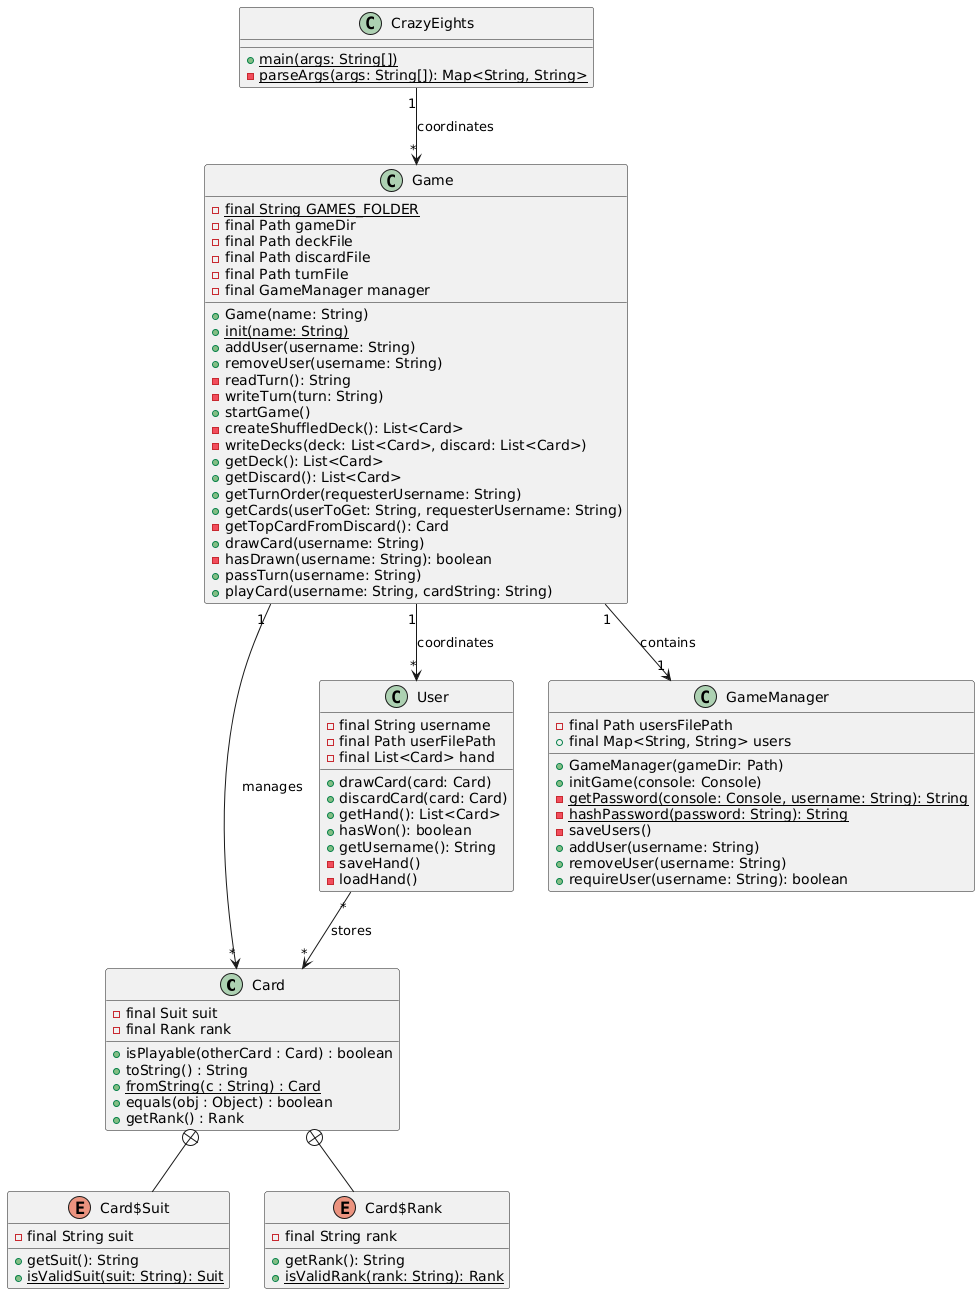
\includegraphics[width=0.8\linewidth]{class/diagram.png}
    \caption{Class Diagram of the Crazy Eights Game}
    \label{fig:class_diagram}
\end{figure}

In figure \ref{fig:class_diagram}, we can see the class diagram of the Crazy Eights game. The diagram illustrates the relationships between different classes, including the Game, User, Card, and Deck classes. Each class has its own attributes and methods, which are used to implement the game logic.

\subsection{CrazyEights Class}
The CrazyEights class is the main entry point of the program. It handles command-line arguments to coordinate the game flow. The class is responsible for validating user input, and invoking methods from other classes to perform specific actions.

\subsection{Game Class}
The Game class represents the game itself. It manages the game state, including the players, deck of cards, and the discard pile. The class provides methods to add or remove players, start the game, and handle player actions such as playing a card or drawing from the deck. In essence it contains the game logic and rules, thus acting as the brain; managing the game state with the turn file, the players file, and the decks files. The class also ensures that the game is played fairly by enforcing the rules of Crazy Eights.

\subsection{User Class}
The User class represents a player in the game. It contains information about the player's name, hand of cards, and their current status in the game. The class provides methods to add or remove cards from the player's hand, check if the player has won, and display the player's hand. In addition, this class is responsible for managing the player's actions, such as playing a card or drawing from the deck; and demonstrating those actions on the actual files for each respective player.

\subsection{Card Class}
The Card class represents a playing card in the game. It contains information about the card's rank and suit. The class provides methods to compare cards, check if a card is playable, and display the card's information. The class also ensures that the cards are represented correctly and can be easily manipulated during the game.

\subsection{GameManager Class}
The GameManager class is responsible for managing the security aspects of the game. It handles user authentication, authorization, and input validation. The class ensures that only authorized users can perform certain actions in the game, such as starting a new game or playing a card. This class is crucial for maintaining the integrity and security of the game.

\section{Run-time Demo}
The Crazy Eights game can be run in a terminal or command prompt. The user can interact with the game by entering commands to perform various actions, such as starting a new game, adding or removing players, and playing cards. A quick demo of the run-time interface is shown in the \href{https://youtu.be/vTJYHRKo5vw}{Crazy Eights Demo Video}. The video demonstrates how to compile and run some of the commands in the game.

\section{AI Disclosure Segment}
The project was developed with the help of GitHub copilot, which is an AI-powered code completion tool. The tool was used to help generate  the class diagram, and performing certain tedious actions. Overall, the AI tool was helpful in speeding up the development but was not relied upon for the logic of this project instead it was used to help with the boilerplate code and repetitive tasks. The final implementation was thoroughly reviewed and tested to ensure that it met the project objectives and security requirements.

\section{Conclusion}
In conclusion, the Crazy Eights game was successfully implemented in Java with a focus on security and object-oriented programming principles. The project met its objectives of understanding data storage techniques, and becoming proficient system programmers. The game provides a fun and engaging way to learn about programming concepts while ensuring that security is a top priority.

\end{document}